\begin{tikzpicture}[
		every node/.append style={draw=gray!80,align=center,minimum width=90pt,very thin}
  	]
	\node (I) at (-3.5,-1.5) {
		\textbf{\small Inicio}
	};
	\node (CB) at (-3.5,0.5) {
		\textbf{\small Cadena de Búsqueda}\\{\scriptsize (gamif* OR rol* game) AND}\\
		{\scriptsize (motivation) OR (gamif* AND rol* game)}\\
		{\scriptsize LIMIT(10 year),}\\
		{\scriptsize AREA(social sciences AND psychology)}
	};
	\node (BD) at (-3.5,4) {
		\textbf{\small Base de Datos}\\{\scriptsize Science direct, Springer link, Scopus,}\\{\scriptsize Oxford Academic, google scholar, EBSCO, UT}
	};
	\node (WC) at (2.7,0.5) {
		\textbf{\small Nubes de Palabras}\\ \includegraphics[width=.3\textwidth]{img/keywords_count_full}
	};
	\node (E) at (2.7,4) {
		\textbf{\small Descarga Articulo/Metadatos}\\{\scriptsize Título, Autores, Resumen, Año,}\\{\scriptsize Palabras Clave, Tipo, Publicación}
	};
	\node (R) at (5.7,5.5) {
		\textbf{\small Artículos recomendados (IA)}
	};
	\node (C) at (8,4) {
		\textbf{\small Clasificación (Jabref)}\\{\scriptsize Review, Gamificación, Narración,}\\{\scriptsize RPG, Motivación, Misceláneo}
	};
	\node (A) at (8,2.3) {
		\textbf{\small Anotación}
	};
	\node (An) at (8,0) {
		\textbf{\small Análisis}\\ 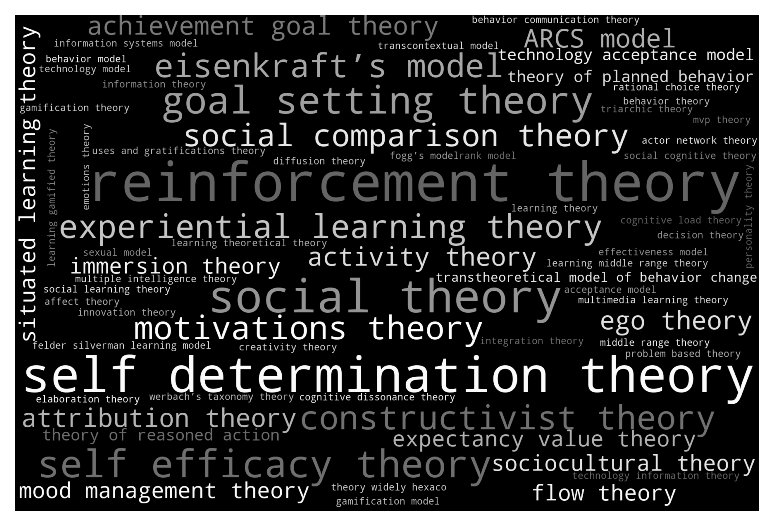
\includegraphics[width=.2\textwidth]{img/teoriasYmodelos.sort}
	};
	\draw[-triangle 90] (I) edge (CB);
	\draw[-triangle 90] (CB) edge (BD);
	\draw[-triangle 90] (BD) edge (E);
	\draw[-triangle 90] (E) edge (WC);
	\draw[-triangle 90] (WC) edge (CB);
	\draw[-triangle 90] (E) edge (C);
	\draw[-triangle 90] (C) edge (A);
	\draw[-triangle 90] (A) edge (An);
	\draw[-triangle 90,dashed] (E) edge (R);
	\draw[-triangle 90,dashed] (R) edge (C);
\end{tikzpicture}

